%% LaTeX-Beamer template for KIT design
%% by Erik Burger, Christian Hammer
%% title picture by Klaus Krogmann
%%
%% version 2.1
%%
%% mostly compatible to KIT corporate design v2.0
%% http://intranet.kit.edu/gestaltungsrichtlinien.php
%%
%% Problems, bugs and comments to
%% burger@kit.edu

\documentclass[18pt]{beamer}
\usepackage[utf8x]{inputenc}
\usepackage{units}
\usepackage{booktabs}

%% CUSTOM
\usepackage{amsmath}
\usepackage{algpseudocode}

%% Definitions
\DeclareMathOperator{\div2}{div}
\renewcommand{\algorithmicrequire}{\textbf{Input:}}
\renewcommand{\algorithmicensure}{\textbf{Output:}}
\algnewcommand\algorithmicto{\textbf{to}}
\algrenewtext{For}[3]{\algorithmicfor\ $#1 \gets #2$ \algorithmicto\ $#3$ \algorithmicdo}
\algnewcommand\algorithmicod{\textbf{od}}
\algrenewtext{EndWhile}{\algorithmicod}
\algrenewtext{EndFor}{\algorithmicod}
%\AtBeginSection[]{%
%\begin{frame}<beamer> % do nothing in handouts
%    \frametitle{Überblick}
%    \tableofcontents[sectionstyle=show/shaded,
%    subsectionstyle=show/show/hide]
%\end{frame}
%}
%\AtBeginSubsection[]{%
%\begin{frame}<beamer> % do nothing in handouts
%    \frametitle{Überblick}
%    \tableofcontents[sectionstyle=show/shaded,
%    subsectionstyle=show/shaded/hide]
%\end{frame}
%}

%% SLIDE FORMAT

% use 'beamerthemekit' for standard 4:3 ratio
% for widescreen slides (16:9), use 'beamerthemekitwide'

\usepackage{templates/beamerthemekit}
%\usepackage{templates/beamerthemekitwide}

 %% TITLE PICTURE

 % if a custom picture is to be used on the title page, copy it into the 'logos'
 % directory, in the line below, replace 'mypicture' with the 
 % filename (without extension) and uncomment the following line
 % (picture proportions: 63 : 20 for standard, 169 : 40 for wide
 % *.eps format if you use latex+dvips+ps2pdf, 
 % *.jpg/*.png/*.pdf if you use pdflatex)


 \titleimage{banner}
 
 
%% Define some colors:
\definecolor{darkblue}{rgb}{0,0,.5}
\definecolor{darkgreen}{rgb}{0,.5,0}

 %% TITLE LOGO

 % for a custom logo on the front page, copy your file into the 'logos'
 % directory, insert the filename in the line below and uncomment it

\titlelogo{logo_150x150}
 
 % (*.eps format if you use latex+dvips+ps2pdf,
 % *.jpg/*.png/*.pdf if you use pdflatex)
 
 %% TikZ INTEGRATION
 
 % use these packages for PCM symbols and UML classes
 % \usepackage{templates/tikzkit}
 % \usepackage{templates/tikzuml}
 
 % the presentation starts here
 
\author{Dominik Muth - dominik.muth@student.kit.edu}
\institute{Institut f\"ur Informatik}

\subtitle{Foliensatz 12}
\date{24. Januar 2013}

\newcommand{\sq}{$\square$}
\newcommand{\da}{$\downarrow$}

\begin{document}

\begin{frame}
    \titlepage
\end{frame}

\begin{frame}{Outline/Gliederung}
    \tableofcontents
\end{frame}

\section{Wiederholung}
\section{Turingmaschinen}
\begin{frame}{Partielle Funktionen}
    \begin{block}{Definition: Partielle Funktion}
        Eine partielle Funktion ist eine rechtseindeutige Relation, die nicht zwingend linkstotal ist.\\
        Wir schreiben
        \begin{align*}
            f: M\dashrightarrow M'
        \end{align*}
    \end{block}
    \begin{columns}[t]
        \begin{column}{.5\textwidth}
            Anschaulich:\\
            Funktionen, die an manchen Stellen ``Definitionslücken'' haben dürfen.\\
            Beispiel:\\
            $\frac{1}{x^2}$ ist eine partielle Funktion ($x=0$ hat keinen Funktionswert)
        \end{column}
        \begin{column}{.5\textwidth}
            \begin{figure}[t]
                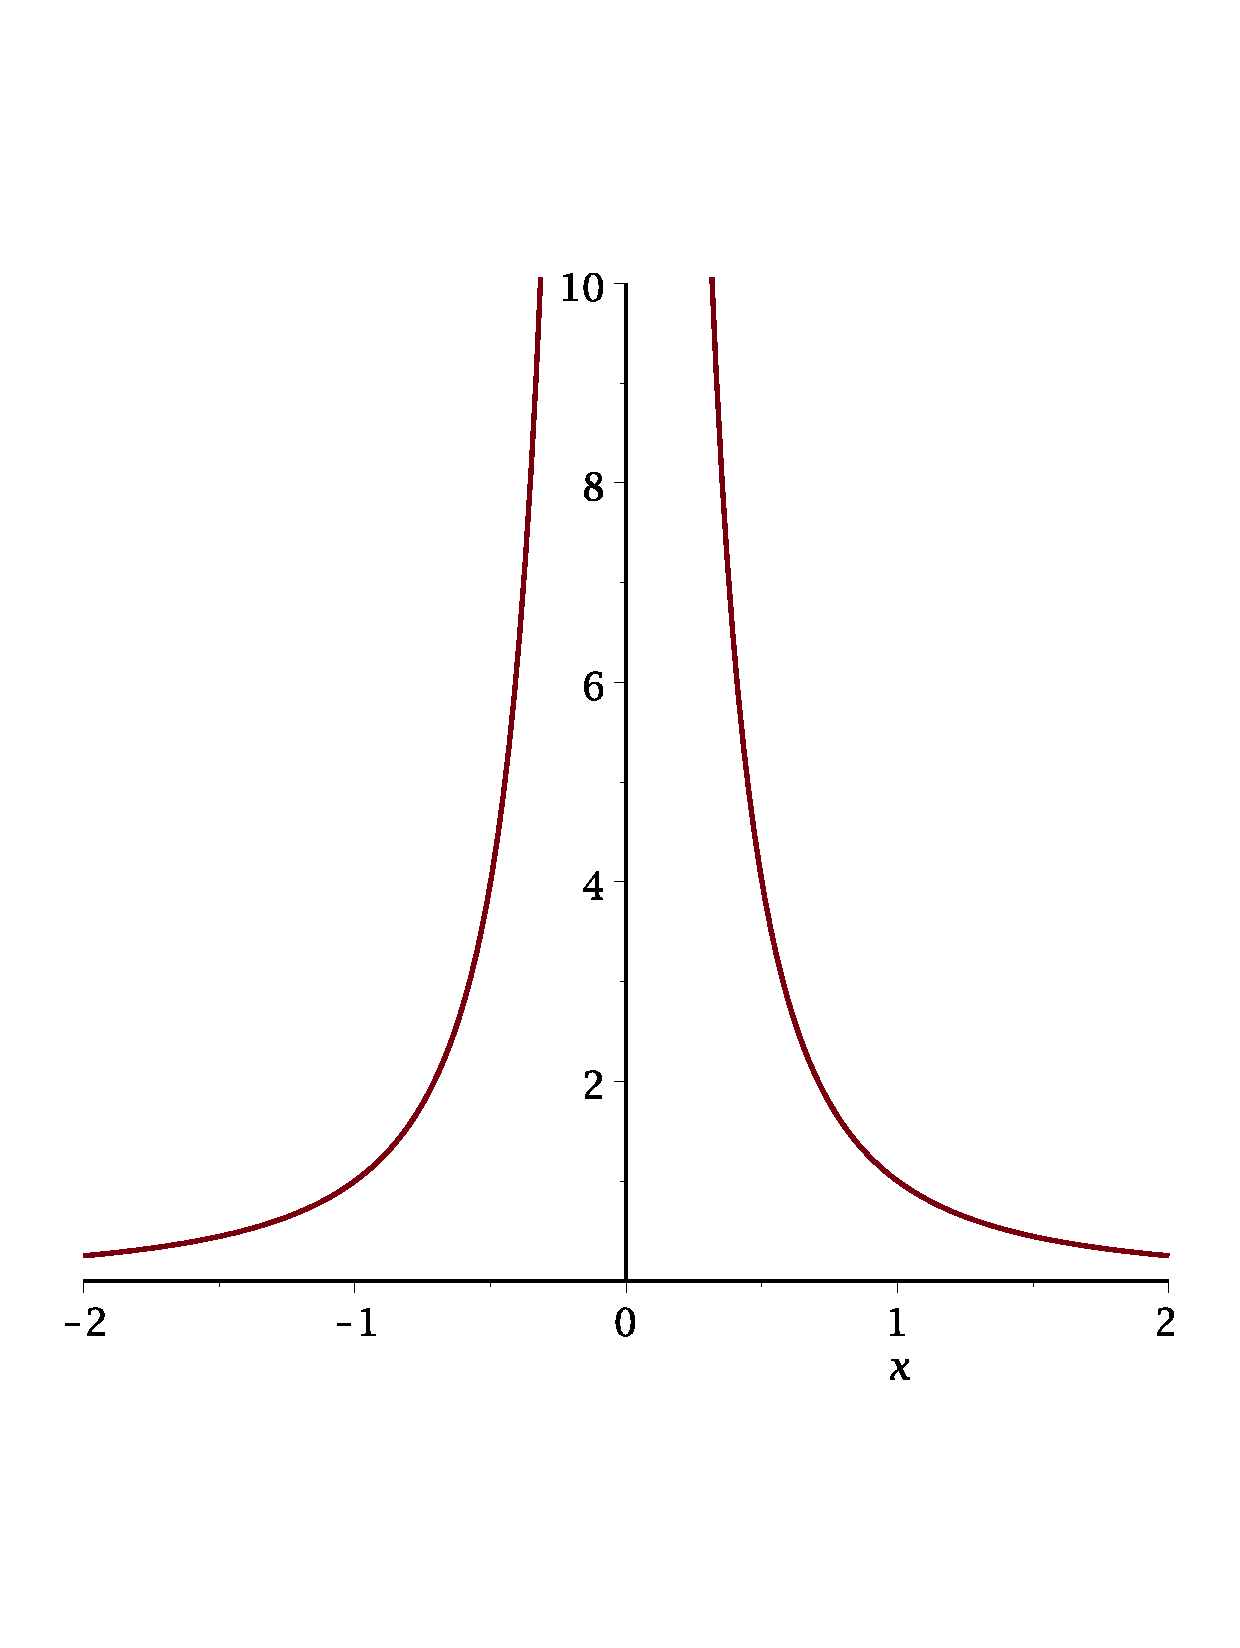
\includegraphics[scale=0.15]{graphics/12/partielle_funktion}
            \end{figure}
        \end{column}
    \end{columns}
\end{frame}
\begin{frame}{Turingmaschine}
    \begin{block}{Definition: Turingmaschine}
        Eine Turingmaschine $T$ ist definiert durch
        \begin{align*}
            T = \left( Z, Z_0, X, f, g, m \right)
        \end{align*}
        Dabei ist 
        \begin{itemize}
            \item $\mathbf{Z}$: die Zustandsmenge
                \pause
            \item \visible<2->{$\mathbf{z_0}$: der Anfangszustand}
                \pause
            \item \visible<3->{$\mathbf{X}$: das Bandalphabet}
                \pause
            \item \visible<4->{$\mathbf{f: Z\times X \dashrightarrow Z}$: die partielle Zustandsüberführungsfunktion}
                \pause
            \item \visible<5->{$\mathbf{g: Z\times X \dashrightarrow g}$: die partielle Ausgabefunktion}
                \pause
            \item \visible<6->{$\mathbf{m: Z\times X \dashrightarrow \left\{ -1, 0, 1 \right\}}$: die partielle Bewegungsfunktion}
        \end{itemize}
    \end{block}
\end{frame}
\begin{frame}{Turingmaschine: Verständnis}
    \textbf{Woher kennen wir ähnliche Funktionen wie $f$ und $g$?}\\
    \pause
    \visible<2->{Von Automaten und Akzeptoren.}\\
    \pause
    \visible<3->{\textbf{Wo war dort der Unterschied?}}\\
    \pause
    \visible<4->{Bei Automaten und Akzeptoren waren die Funktionen nicht partiell.}\\
    \pause
    \visible<5->{\textbf{Was bewirken partielle Zustandsübergangsfunktionen?}}\\
    \pause
    \visible<6->{Die partiellen Funktionen bewirken, dass der Automat zu manchen \textit{Konfigurationen} stehen bleibt.}
    \begin{figure}
        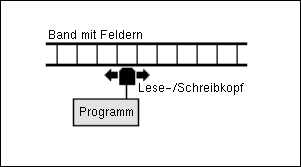
\includegraphics[scale=0.6]{graphics/12/Turingmaschine.png}
    \end{figure}
\end{frame}
\begin{frame}{Konfiguration einer Turingmaschine}
    \begin{block}{Definition: Konfiguration}
        Eine Turingmaschine befindet sich zu jedem Zeitpunkt in einem ``Gesamtzustand'', den wir eine Konfiguration nennen. Sie ist beschrieben durch
        \begin{itemize}
            \item den aktuellen Zustand $z \in Z$ der Steuereinheit
            \item die aktuelle Beschriftung $b\in X^*$ des gesamten Bandes
            \item die aktuelle Position $p \in \mathbb{Z}$ des Kopfes
        \end{itemize}
    \end{block}
\end{frame}
\begin{frame}{Turingmaschine: Beispiel}
    \begin{figure}
        \centering
    \begin{tikzpicture}[shorten >=1pt,initial text=,node distance=2cm,auto,->,>=stealth,baseline=(B.base)]
        % \node[state,initial]  (S)                       {$S$};
        \node[state,initial]  (A)          {$A$};
        % \node (nix) [right of=A] {};
        \node[state]          (B) [above right of=A] {$B$};
        \node[state]          (C) [right of=B] {$C$};
        \node[state]          (E) [right of=A] {$E$};
        \node[state]          (D) [right of=E] {$D$};
        \path[->]
        % (S) edge              node  {$\square|\squareR$} (A)
        (A) edge              node  {$1| XR$} (B)
        (B) edge [loop above] node  {$1| 1R$} ()
        edge              node  {$\square |\square R$} (C)
        (C) edge [loop above] node  {$1| 1R$} ()
        edge              node  {$\square | 1L$} (D)
        (D) edge [loop below] node  {$1| 1L$} ()
        edge              node  {$\square |\square L$} (E)
        (E) edge [loop below] node  {$1| 1L$} ()
        edge              node  {$X| 1R$} (A)
        ;
    \end{tikzpicture}
\end{figure}
    \begin{table}
        \begin{tabular}{lccccc}
        \toprule
                  & A     & B             & C         & D                 & E \\
        \midrule
        $\square$ &       & C,$\square$,R & D,1,L     & E,$\square$,L     &  \\
        1         & B,X,R & B,1,R         & C,1,R     & D,1,L             & E,1,L \\
        X         &       &               &           &                   & A,1,R \\
        \bottomrule
        \end{tabular}
    \end{table}
\end{frame}
\begin{frame}{Turingmaschine: Beispiel}
    \textbf{Was macht die Turingmaschine?}\\
    Was passiert mit dem Wort $\dots\square 11\square\dots$, das auf dem Band steht?
    \begin{table}
        \begin{tabular}{lcccccccc}
            \hline
               &     & A   &     &     &     &     &     &     \\
             1.&     & \da &     &     &     &     &     &     \\
               & \sq & 1   &  1  & \sq & \sq & \sq & \sq & \sq \\
           \hline\visible<2->{
               &     &     &  B  &     &     &     &     &     \\
             2.&     &     & \da &     &     &     &     &     \\
               & \sq & X   &  1  & \sq & \sq & \sq & \sq & \sq \\
           \hline}\visible<3->{
               &     &     &     & B   &     &     &     &     \\
             3.&     &     &     & \da &     &     &     &     \\
               & \sq & X   &  1  & \sq & \sq & \sq & \sq & \sq \\
           \hline}\visible<4->{
               &     &     &     &     &  C  &     &     &     \\
             4.&     &     &     &     & \da &     &     &     \\
               & \sq & X   &  1  & \sq & \sq & \sq & \sq & \sq \\}
        \end{tabular}
    \end{table}
\end{frame}
\begin{frame}
    \begin{table}
        \begin{tabular}{lcccccccc}
           \hline
               &     &     &     &  D  &     &     &     &     \\
             5.&     &     &     & \da &     &     &     &     \\
               & \sq & X   &  1  & \sq & 1   & \sq & \sq & \sq \\
           \hline\visible<2->{
               &     &     &  E  &     &     &     &     &     \\
             6.&     &     & \da &     &     &     &     &     \\
               & \sq & X   &  1  & \sq & 1   & \sq & \sq & \sq \\
           \hline}\visible<3->{
               &     &  E  &     &     &     &     &     &     \\
             7.&     & \da &     &     &     &     &     &     \\
               & \sq & X   &  1  & \sq & 1   & \sq & \sq & \sq \\
           \hline}\visible<4->{
               &     &     &  A  &     &     &     &     &     \\
             8.&     &     &\da  &     &     &     &     &     \\
               & \sq & 1   &  1  & \sq & 1   & \sq & \sq & \sq \\
           \hline}\visible<5->{
               &     &     &     &  B  &     &     &     &     \\
             9.&     &     &     & \da &     &     &     &     \\
               & \sq & 1   &  X  & \sq & 1   & \sq & \sq & \sq \\
           \hline}\visible<6->{
               &     &     &     &     &  C  &     &     &     \\
            10.&     &     &     &     & \da  &     &     &     \\
               & \sq & 1   &  X  & \sq & 1   & \sq & \sq & \sq \\}
        \end{tabular}
    \end{table}
\end{frame}
\begin{frame}
    \begin{table}
        \begin{tabular}{lcccccccc}
           \hline
               &     &     &     &     &     &  C  &     &     \\
            11.&     &     &     &     &     & \da &     &     \\
               & \sq & 1   &  X  & \sq & 1   & \sq & \sq & \sq \\
           \hline\visible<2->{
               &     &     &     &     &  D  &     &     &     \\
            12.&     &     &     &     & \da &     &     &     \\
               & \sq & 1   &  X  & \sq & 1   & 1 & \sq & \sq \\
           \hline}\visible<3->{
               &     &     &     &  D  &     &     &     &     \\
            13.&     &     &     & \da &     &     &     &     \\
               & \sq & 1   &  X  & \sq & 1   & 1 & \sq & \sq \\
           \hline}\visible<4->{
               &     &     &  E  &     &     &     &     &     \\
            14.&     &     & \da &     &     &     &     &     \\
               & \sq & 1   &  X  & \sq & 1   & 1 & \sq & \sq \\
           \hline}\visible<5->{
               &     &     &     & A   &     &     &     &     \\
            15.&     &     &     & \da &     &     &     &     \\
               & \sq & 1   &  1  & \sq & 1   & 1 & \sq & \sq \\}
        \end{tabular}
    \end{table}
\end{frame}
\begin{frame}{Turingmaschine: Beispiele}
    Nicht jede Turingmaschine kommt wie die vorherige zum Halten. Es gibt auch unendliche Berechnungen (wie in Java).
    \begin{block}{Turingmaschine als Akzeptor}
        Ist eine Turingmaschine ein Akzeptor, so ist ein Eingabewort akzeptiert, wenn der Endzustand ein akzeptierter Zustand ist.
    \end{block}
    \begin{block}{Definition: Eigenschaften von Sprachen}
        Eine Sprache $L$ ist
        \begin{itemize}
            \item eine aufzählbare Sprache, wenn es eine Turingmaschine gibt, die $L$ akzeptiert oder
            \item eine entscheidbare Sprache, wenn es eine Turingmaschine gibt, die $L$ akzeptiert und immer hält.
        \end{itemize}
    \end{block}
\end{frame}
\begin{frame}{Turingmaschine als Akzeptor: Beispiel}
    \begin{figure}
        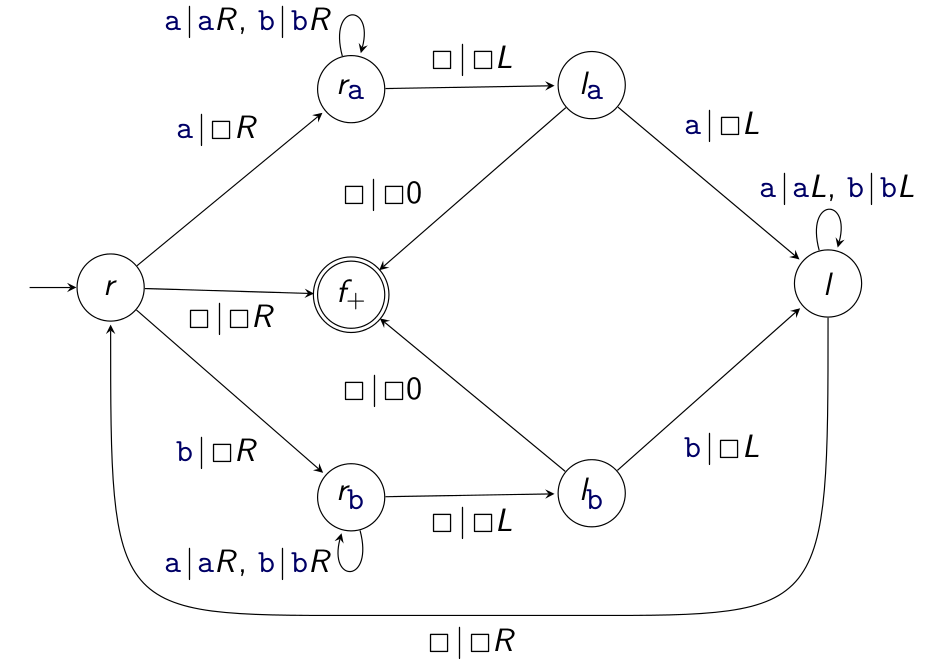
\includegraphics[scale=0.3]{graphics/12/palindrom.png}
    \end{figure}
    Was macht diese Turingmaschine?
\end{frame}
\begin{frame}{Klausuraufgabe}
    TODO
\end{frame}
\section{Alan Turing}
\begin{frame}{Alan Turing}
    \begin{columns}
        \begin{column}{.7\textwidth}
            \begin{itemize}
                \item Verantwortlich für viele wichtige Entwicklungen in der theoretischen Informatik
                \item Mitentwickler der \emph{Turing-Bombe}, die im zweiten Weltkrieg zur Entschlüsselung der Enigma half
                \item nebenbei auch guter Marathonläufer\\(nahm an Olympiavorwettkämpfen teil)
                \item wurde wegen Homosexualität 1952 einer psychiatrischen Zwangsbehandlung unterzogen
                \item musste dabei weibliche Hormone nehmen
                \item Depression führten zu Selbstmord
            \end{itemize}
        \end{column}
        \begin{column}{.3\textwidth}
            \begin{figure}
                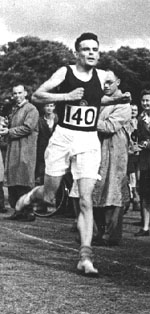
\includegraphics[scale=0.7]{graphics/12/turing.jpg}
            \end{figure}
        \end{column}
    \end{columns}
\end{frame}

\end{document}
